% !TEX encoding = UTF-8
% !TEX TS-program = pdflatex
% !TEX root = ../Relazione.tex
% !TEX spellcheck = it-IT

%%%%%%%%%%%%%%%%%%%%%%%%%%%%%%%
\section{Going beyond GPS localization}
\label{sec:gps}
%%%%%%%%%%%%%%%%%%%%%%%%%%%%%%%

\subsection{GPS and battery drain}
La geolocalizzazione dei dispositivi, soprattutto quelli mobile, sta rapidamente diventando parte intergrante del nostro modo quotidiano di fruire la tecnologia. Si usa nel navigatore stradale, per impostare automaticamente il luogo di cui desideriamo le previsioni del tempo o da cui vogliamo prendere un treno o un aereo, per aggiungere informazioni contestuali alle fotografie che scattiamo e tanto altro ancora.

Il modo storicamente utilizzato per effettuare la geolocalizzazione è per via satellitare, tramite il GPS. Ma il GPS ha due tipi di problemi:

\begin{itemize}
 \item è \emph{davvero} lento ad agganciare un numero congruo di satelliti, tali da poter registrare una posizione accurata,
 \item consuma un ingente consumo di energia. 
\end{itemize}

Soprattutto il secondo punto è in palese conflitto con l'esigenza dei moderni dispositivi portatili di avere un'ampia autonomia energerica. Per porre rimedio a questo fatto, Google ha via via comiciato ad utilizzare altri tipi alternativi di geolocalizzazione, per comporre un sistema ibrido.

\begin{enumerate}
 \item Un primo grado di grossolana geolocalizzazione avviene tramite le celle della rete telefonica, a cui tutti gli smartphone sono connessi. La precisione è dell'ordine delle centinaia di metri.
 \item Un secondo grado, molto più accurato, viene realizzato tramite le reti wifi visibili in quell'istante dal dispositivo. La precisione è dell'ordine di qualche decina di metri.
 \item Infine, solo se il compito richiesto richiede una precisione ulteriore, si accende il GPS, per un risultato con la precisione inferiore al metro. Cominciare da una stima della posizione più che accettabile riduce di molto la durata delle operazioni a GPS acceso, consentendo un drastico risparmio della batteria.
\end{enumerate}

\subsubsection*{Geolocalization via WiFi}
La diffusione del Wifi è ormai capillare, soprattutto in contesto cittadino. Virtualmente c'è un router WiFi in ogni appartamento. Mentre camminiamo per la città con il WiFi dello smartphone acceso, captiamo in ogni punto decine di segnali. Se sono note la posizione di questi router e la potenza del segnale da loro emesso, è possibile triangolare la nostra posizione con una notevole precisione. Ciò è dovuto sia al fatto che un segnale WiFi ha un raggio tipico di una trentina di metri, sia per l'ingente numero di segnali con i quali si sta triangolando, tipicamente più di una decina.

Quindi per sapere la mia posizione devo avere accesso a una mappa delle posizioni di tutti i router. E come si costruisce questa mappa? Esattamente al contrario: camminando per la città con GPS acceso, avendo dunque un'alta precisione sulla posizione del dispositivo, e triangolando la posizione di tutti i router visibili combinando tutte le rilevazioni del tracciato.

Dunque Google ha mappato tutti i WiFi di tutto il globo per dare la possibilità agli utenti dei suoi servizi come Google Maps (e delle applicazioni che si appoggiano alle sue API) di ottenere la propria localizzazione con una buona precisione e un consumo di batteria risibile. La precisione è arrivata ad essere dell'ordine dei 5 metri e i tempi di accesso pressoché istantanei: di fatto rendendo inutile accendere il GPS nella maggior parte dei casi.

Questo tipo di localizzazione ha inoltre un altro grande vantaggio: funziona anche sottoterra e dentro gli edifici, luoghi normalmente inaccessibili al segnale GPS, di natura satellitare.

Ovviamente la mappa dei router WiFi è in continua evoluzione, per cui il modo più conveniente per redigerla è sfruttando il crowdsourcing: ai milioni di utenti ignari, giornalmente in moto per la città, viene acceso il GPS un paio di volte al giorno per pochi secondi, in un momento di inutilizzo del dispositivo, e in questo modo si crea velocemente una mappa complessiva e quotidianamente aggiornata, a beneficio di tutti.

Tutto questo è tremendamente intelligente ed efficiente. C'è un solo grande problema: i dati sono chiusi.

\subsection{Mozilla Location Service}
\begin{wrapfloat}{figure}{I}{0pt}
	\centering
	
\includegraphics[width=0.3\textwidth]{./Immagini/Dati/MLSlogo.png}
	\caption{Logo del MLS}
\end{wrapfloat}
Mozilla è da sempre impegnata nello sviluppo di tecnologie web aperte e standardizzate. Avendo riconosciuta la centralità della geolocalizzazione e la crescita esponenziale di siti ed applicazioni location-aware, ha deciso di ricalcare le orme di Google e fondare il suo servizio di geolocalizzazione usando WiFi ed antenne cellulari: \citetitle{mozilla}.


L'obbiettivo è quello di geolocalizzare gli utenti sulla base dell'ambiente radio che li circonda: MLS è un progetto collaborativo per creare un database mondiale aperto di Cell ID e WiFi georeferenziati. La mappatura viene fatta dagli utenti su base puramente volontaria, utilizzando l'apposita applicazione \emph{Mozilla Stumbler}.

\begin{figure}[ht!]
	\centering
	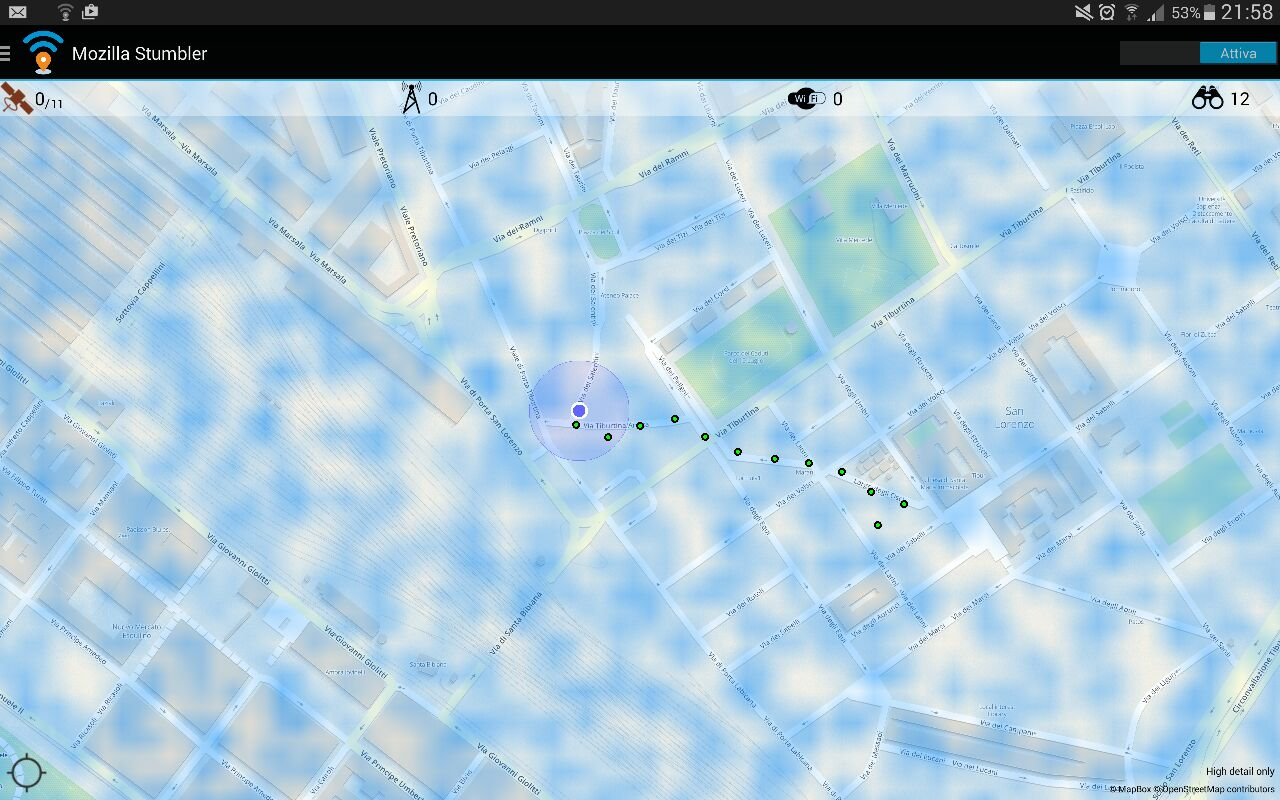
\includegraphics[width=0.8\textwidth]{./Immagini/Dati/appmap.jpg}
	\caption{\emph{Screen} dell'applicazione attiva}
	\label{fig:mapp}
\end{figure}
Il progetto è ormai maturo e, come si può osservare nelle mappe in fig. \ref{fig:mapp} e \ref{fig:wapp} la copertura del mondo è molto capillare.
\begin{itemize}
	\item La prima mostra un esempio di utilizzo del programma a San Lorenzo, in un normale percorso cittadino. I pallini verdi sono i punti GPS delle rilevazioni complete (WiFi + rete cellulare) effettuate durante il tragitto. Come si può notare sono piuttosto fitti: 4 o 5 per ogni isolato. Le aree sfumate in blu mostrano invece, in maniera approssimata per motivi di privacy, l'esito dell'eleborazione di tutte le precedenti osservazoni nell'area, ovvero tutti i router WiFi e le antenne ricostruiti fin ora. La mappa è fittissima, ma questo non deve trarre in inganno: è ancora incompleta e per certi versi inaffidabile. Un esempio diretto sono le numerose ricostruzioni che appaiono in mezzo ai binari della stazione Termini: quelle derivano dai WiFi all'interno dei treni a cui si collegano i viaggiatori, ma che essendo oggetti in moto non possono essere usati ai fini della geolocalizzazione e pertanto dovrebbero essere filtrati ed esclusi dal database.
	\item La seconda mappa (interattiva) mostra invece la copertura globale raggiunta dal progetto. Sebbene risulti uno stadio abbastanza avanzato, si può notare come ci siano ancora delle disparità di mappatura anche tra gli stati ad alta presenza tecnologica: si confrontino ad esempio le capitali della Cina e del Giappone. Inoltre, essendo un progetto collaborativo open source e con sede negli Stati Uniti, sì può vedere come gli stati in cui la cultura open è meno diffusa o quelli in tensione con gli USA per quanto riguarda la politica estera risultino globalmente meno mappati. Un esempio emblematico potrebbe essere la differenza tra Nord Korea e Sud Korea.
\end{itemize}

\begin{figure}[b!]
	\centering
	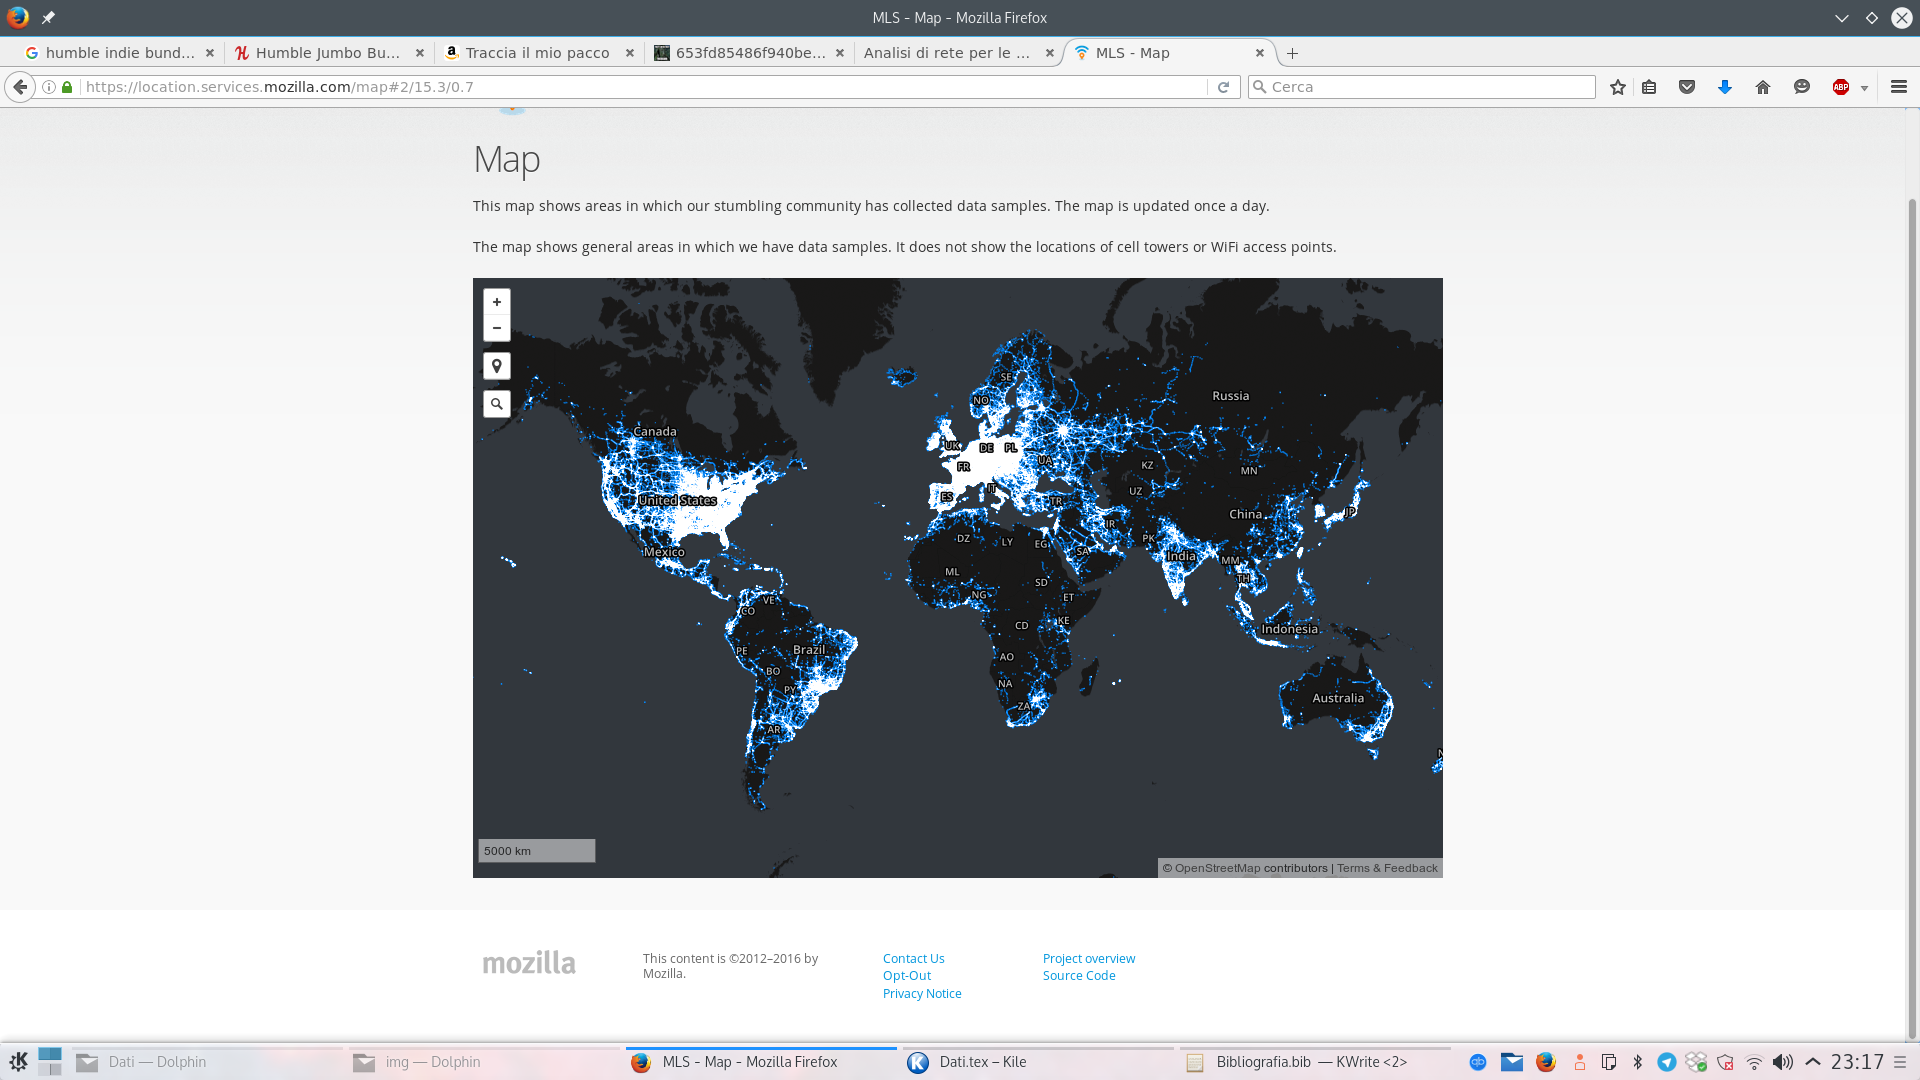
\includegraphics[width=0.8\textwidth]{./Immagini/Dati/MLSmap.png}
	\caption{Immagine della mappa fornita da Mozilla}
	\label{fig:wapp}
\end{figure}

Dato l'approccio di \emph{crouwdsourcing} collaborativo, i dati sono tanti e a copertura mondiale, continuamente aggiornati, aperti, facilmente scaricabili in database ordinati, puliti e ben documentati. In Tabella \ref{tab:statacq} sono elencate alcune statistiche per avere un'idea dei numeri in gioco:
\begin{table}[t]
\centering
\caption{Alcune statistiche dei dati forniti da MLS}
\parbox{0.45\textwidth}{
\centering
	\begin{tabular}{cc}
	\toprule
	data 				&total\\
	\midrule
	Wifi Networks 			&521.610.000\\
	Wifi Observations 		&1.1006.560.000\\
	MLS Cells 			&20.390.000\\
	MLS Cell Observations 	&2.468.460.000\\
	OpenCellID Cells 		&7.990.000\\
	\midrule
	\end{tabular}
\label{tab:statacq}
}
\\
\parbox{0.45\textwidth}{
\centering
	\begin{tabular}{ccc}
	network 		&Italy 		&United States\\
	\midrule
	GSM (2G) 		&132.468 		&230.236\\
	UMTS (3G) 	&516.379 		&976.603\\
	LTE (4G) 		&96.489 		&1.595.402\\
	Total Cells 	&745.336 		&2.802.241\\
	WiFis 		&9.844.682 	&175.599.375\\
	\bottomrule
	\end{tabular}
\label{tab:statreg}
}
\label{tab:expectedfluoZnSe}
\end{table}

Mozilla Location Service funziona sia con le antenne cellulari che con i WiFi, soltanto che attulamente i dati della mappa WiFi (mostrati approssimati nella mappa precedente) non possono essere resi pubblici per questioni relative alle norme sulla privacy vigenti sia negli Stati Uniti sia in altre nazioni.

Pertanto gli unici dati attualmente liberamente disponibili (dominio pubblico, licenza CC0) sono quelli sulle antenne radio delle varie generazioni: 2G (GSM), 3G (UMTS), 4G (LTE).
I dati forniti da Mozilla sono un'estensione di quelli già disponibili sulla piattaforma \citetitle{cellid}, anche loro open (licenza CC-BY-SA 3.0).

Questi sono dunque i dati che abbiamo analizzato in questa nostra tesina.

\clearpage
\section{MLS dataset}
\label{sec:mls}
I dati scaricabili dal sito del progetto Mozilla Location Service appaiono come in tabella \ref{tab:esempiodati}; vengono forniti in un file CSV, le cui voci, secondo la documentazione ufficiale, sono organizzate nella seguente maniera:

\begin{description}
 \item[radio] Network type. One of the strings GSM, UMTS or LTE.
 \item[mcc] Mobile Country Code. An integer, for example 505, the code for Australia.
 \item[net] For GSM, UMTS and LTE networks, this is the mobile network code (MNC). An integer, for example 4, the MNC used by Vodaphone in the Netherlands.
 \item[area] For GSM and UMTS networks, this is the location area code (LAC). For LTE networks, this is the tracking area code (TAC). An integer, for example 2035.
 \item[cell] For GSM and LTE networks, this is the cell id or cell identity (CID). For UMTS networks this is the UTRAN cell id, which is the concatenation of 2 bytes of radio network controller (RNC) code and 2 bytes of cell id. An integer, for example 32345.
 \item[unit] For UMTS networks, this is the primary scrambling code (PSC). For LTE networks, this is the physical cell id (PCI). For GSM networks, this is empty. An integer, for example 312.
 \item[lon] Longitude in degrees between -180.0 and 180.0 using the WSG 84 reference system. A floating point number, for example 52.3456789.
 \item[lat] Latitude in degrees between -90.0 and 90.0 using the WSG 84 reference system. A floating point number, for example -10.034.
 \item[range] Estimate of radio range, in meters. This is an estimate on how large each cell area is, as a radius around the estimated position and is based on the observations or a knowledgeable source. An integer, for example 2500.
 \item[samples] Total number of observations used to calculate the estimated position, range and averageSignal. An integer, for example 1200.
 \item[changeable] Whether or not this cell is a position estimate based on observations, and therefore subject to change in the future, or is an exact location entered from a knowledgeable source. A boolean value, encoded as either 1 (for “changeable”) or 0 (for “exact”).
 \item[created] Timestamp of the time when this record was first created. An integer, counting seconds since the UTC Unix Epoch of 1970-01-01T00:00:00Z. For example, 1406204196, which is the timestamp for 2014-07-24T12:16:36Z.
 \item[updated] Timestamp of the time when this record was most recently modified. An integer, counting seconds since the UTC Unix Epoch of 1970-01-01T00:00:00Z. For example, 1406204196, which is the timestamp for 2014-07-24T12:16:36Z.
 \item[averageSignal] Average signal strength from all observations for the cell network. An integer value, in dBm. For example, -72.\\
 This field is only used by the OpenCellID project and historically has been used as a hint towards the quality of the position estimate.
\end{description}

I dati forniti sono di tipo aggregato, ovvero riportano il numero di osservazioni per antenna ed il risultato della stima della sua posizione. Esistono anche dati grezzi, ovvero corrispondenti alle singole osservazioni dei singoli utenti. Tale dataset però non viene reso pubblicamente disponibile, in quanto contenente diverse informazioni, anche di carattere dinamico, utili a tracciare il singolo individuo. È allo studio un meccanismo di autorizzazioni per permettere agli utenti consci degli eventuali rischi di pubblicare i dati che li riguardano.

I valori di latitudine e longitudine, per le coordinate nelle proiezioni geografiche, seguono il sistema di riferimento dettato dalla convenzione \emph{WSG 84 Web Mercator}.

\begin{table}[ht!]
\centering
\caption{Esempio del dataframe MLS}
	\begin{tabular}{ccccccc}
	\toprule
radio 	&mcc 	&net &area 	&cell \\	
GSM 		&262 	&7 	&20205 	&2227 \\	
GSM 		&262 	&2 	&685		&6132 \\	
GSM 		&262 	&1 	&14660 	&39399 \\	
GSM 		&262 	&7 	&20202 	&33063 \\
GSM 		&262 	&7 	&20205 	&2472 \\
\midrule
unit 		 &lon	&lat 		&range 	&samples \\
NaN		&13.308816 	&52.512122	&147481 	&14586 \\
NaN		&7.018766 	&49.223543	&14976 	&5336 \\
NaN		&9.879624 	&51.335388	&101430 	&4049 \\	
NaN		&13.327494	&52.516999	&148854 	&6412 \\	
NaN		&13.296922	&52.507817	&132401 	&11216 \\	
\midrule
changeable 	&created 		&updated 		&averageSignal\\
1 			&1299573448 	&1453335612 	&-64\\
1 			&1299584114 	&1453337312 	&-74\\
1 			&1299693112 	&1453335486 	&-57\\
1 			&1301668631 	&1453335612 	&-61\\
1 			&1301668631 	&1453335612 	&-65\\
\bottomrule
	\end{tabular}
\label{tab:esempiodati}
\end{table}

\subsection{Data selection}
Una volta scaricati i dati aggregati dalla pagina web \lstinline{https://location.services.mozilla.com/downloads} si sono cominciate le operazioni di selezione dei dati. Il data sample riguarda tutti i continenti e risulta molto grosso (un file csv di circa 650 MB), per cui è necessario ridurlo il più possibile per poterlo maneggiare con il nostro limitato quantitativo di RAM.

Una prima grossolana ma efficiente scrematura riguarda i dati caratterizzati da un mobile county code non italiano, si è pertanto imposta la condizione
\begin{lstlisting}
mcc == 222
\end{lstlisting}
Successivamente vengono scartati i dati ritenuti inaffidabili, ovvero con soltanto una rivelazione da parte degli utenti
\begin{lstlisting}
samples > 1
\end{lstlisting}

Adesso che il datasample si è molto ridotto, possiamo effettuare delle operazioni computazionalmente un po' più pesanti: vogliamo eliminare tutte le rilevazioni al di fuori del Grande Raccordo Anulare, che per semplicità è stato schematizzato come una circonferenza di raggio 10 km con centro esattamente nel Colosseo. Per far questo serve definire una nozione di distanza. Dato che i nostri sono dati geolocalizzati sarebbe naturale introdurre una distanza geodesica. A tal fine abbiamo usato la libreria \emph{geopy}, che contiene due definizioni differenti:

\begin{itemize}
 \item \emph{Great circe distance}: la distanza geodesica su una sfera. Per due punti non agli antipodi passa sempre una circonferenza di raggio massimo lungo cui scorre la geodesica, ovvero il cammino di minima distanza.
 \item \emph{Vincenty distance}: la distanza geodesica su un ellissoide oblato. Tale distanza tiene in conto che la Terra non è una sfera perfetta ma è invece leggermente schiacciata ai poli. Delle due è quella più accurata, ma anche quella più difficile da calcolare numericamente.
\end{itemize}
L'ulteriore condizione da soddisfare per i dati risulta dunque
\begin{lstlisting}
geodesicDistance(place) <= raggioRaccordoAnulare
\end{lstlisting}

Si sono fatte differenti prove sia con \lstinline{vincenty} (più lenta) che con \lstinline{great_circle} (leggermente più veloce), ma i tempi di calcolo risultavano comunque spropositati. Pertanto abbiamo fatto una approssimazione: dato che la città di Roma sottende un angolo solido minuscolo rispetto alla totalità del pianeta, abbiamo ritenuto accettabile usare una distanza euclidea, ovviamente trasformando in metri le coordinate angolari di latitudine e longitudine con i relativi fattori di scala, dettati dal raggio terrestre.

La distanza euclidea coinvolge solo quadrati è radici quadrate, risultando nel complesso circa dieci volte più veloce delle altre due concorrenti. Il prezzo da pagare è una leggerissima imprecisione, del tutto trascurabile alle nostre scale. La funzione utilizzata è pertanto
\begin{lstlisting}
def euclideanDistace(x,y):
    return numpy.sqrt(numpy.square(x) + numpy.square(y))
\end{lstlisting}
Da notare il fatto che per il calcolo algebrico è stata utilizzata la libreria \emph{numpy} invece che la libreria \emph{math} built-in in Python, poiché è più veloce (è scritta in C) e supporta le operazioni direttamente su vettori di coordinate.

I dati sono stati importati in un \emph{dataframe} tabulare usando la libreria \emph{pandas}. Questo che ci ha permesso di effettuare facilmente tutte le \emph{query} necessarie per il filtraggio dei dati.
\clearpage

\begin{table}[t]
\caption{Esempio del dataframe da noi utilizzato}
	\begin{tabular}{ccccccccc}
	\toprule
radio	&net &cell 	&lon 	 &lat 		&range 	&samples 	&distance &degree\\
GSM		&10 	&29369 	&12.630353 &41.892274 	&10568 	&2 		&11457 	&2412\\
GSM 		&10 	&28691 	&12.620040 &41.890106 	&9674 	&2 		&10598 	&2361\\
GSM 		&88 	&19451 	&12.531354 &41.986043 	&2172 	&4 		&11129 	&179\\
GSM 		&88 	&16608 	&12.605920 &41.918988 	&4129 	&7 		&9953 	&621\\
GSM 		&88 	&55647 	&12.604219 &41.928254 	&9245 	&23 		&10201 	&2048\\
\bottomrule
	\end{tabular}
\label{tab:datinostri}
\end{table}

A questo punto abbiamo finalmente il nostro datasample della città di Roma: circa 7000 antenne in un file csv agevolmente maneggiabile di circa 1MB.

Per visualizzare agevolmente i nostri dati serve una mappa georeferenziata, preferibilmente interattiva. A tal fine per il notebook di IPython abbiamo usato la libreria \emph{gmaps}, che dà semplice accesso inline alle mappe di Google Maps dando la possibilità di creare una \emph{heatmap}, mentre per l'HTML di questa presentazione abbiamo usato le analoghe funzioni della libreria \emph{gmplot} (per scrivere queste poche linee di codice c'è voluto un intero pomeriggio!):

\begin{lstlisting}
roma = pandas.read_csv("../data/Roma_towers.csv")
coordinate = roma[['lat', 'lon']].values
heatmap = gmaps.heatmap(coordinate)
gmaps.display(heatmap)

colosseo = (41.890183, 12.492369)
mappa = gmplot.GoogleMapPlotter(41.890183, 12.492369, 12)
mappa.heatmap(roma.lat.values,roma.lon.values)
mappa.draw("../doc/heatmap.html")
\end{lstlisting}
\begin{figure}[b!]
	\centering
	\subfloat
	{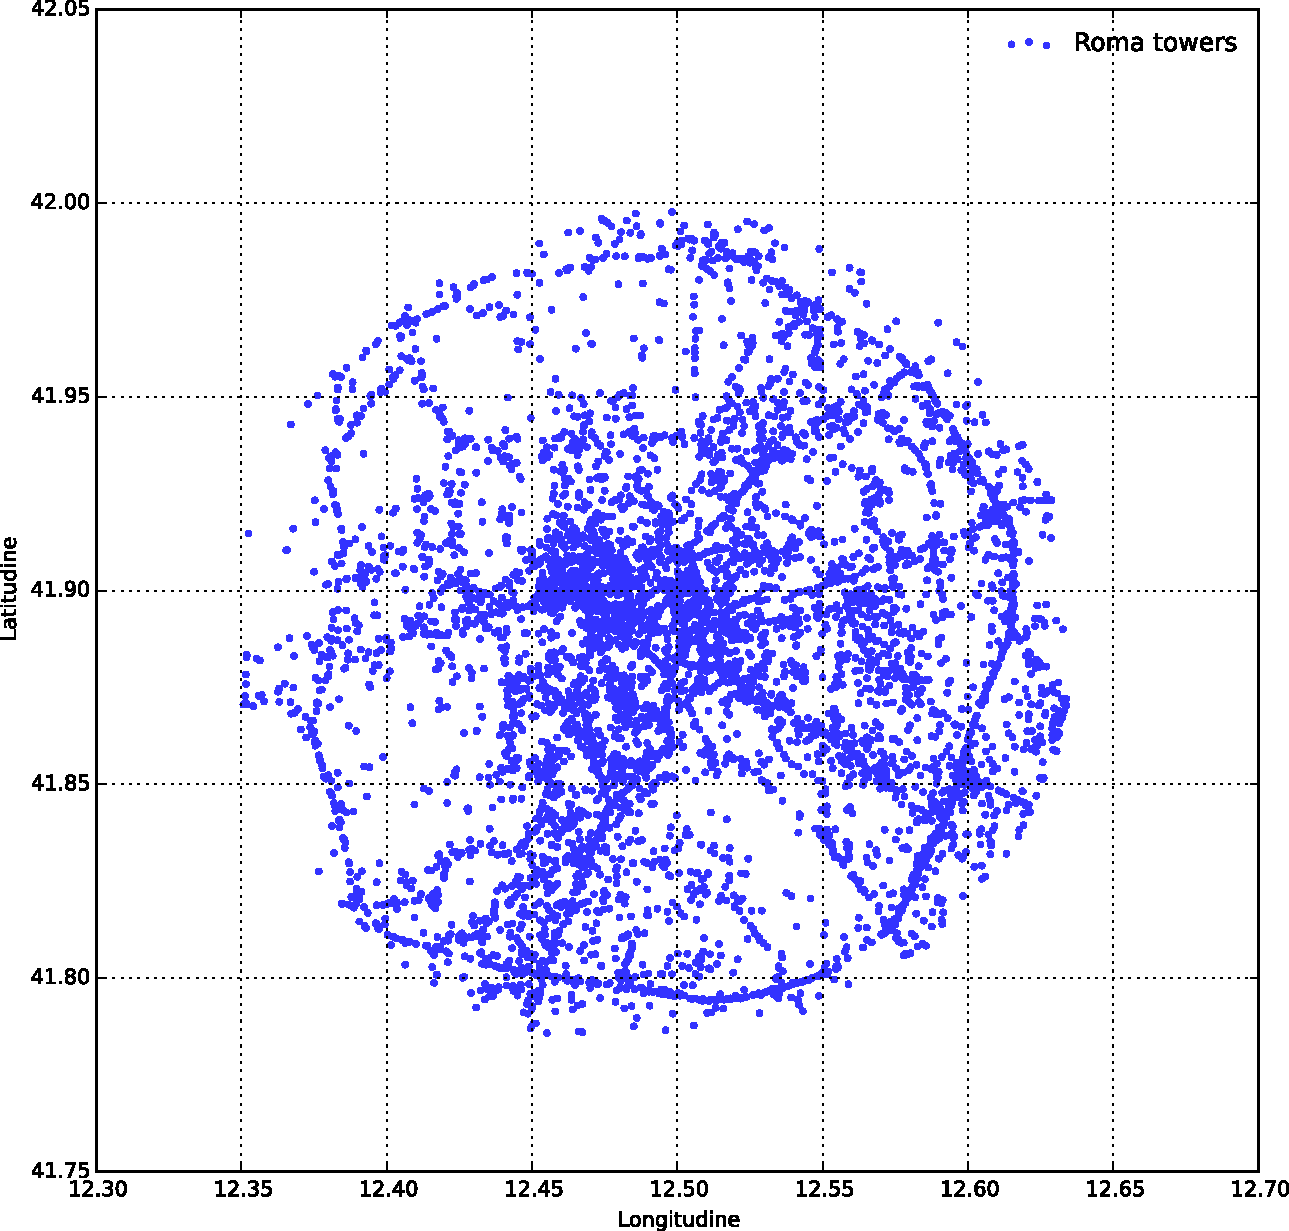
\includegraphics[width=0.5\textwidth]{./Immagini/Dati/roma}}
% 	$\;$
	\subfloat
	{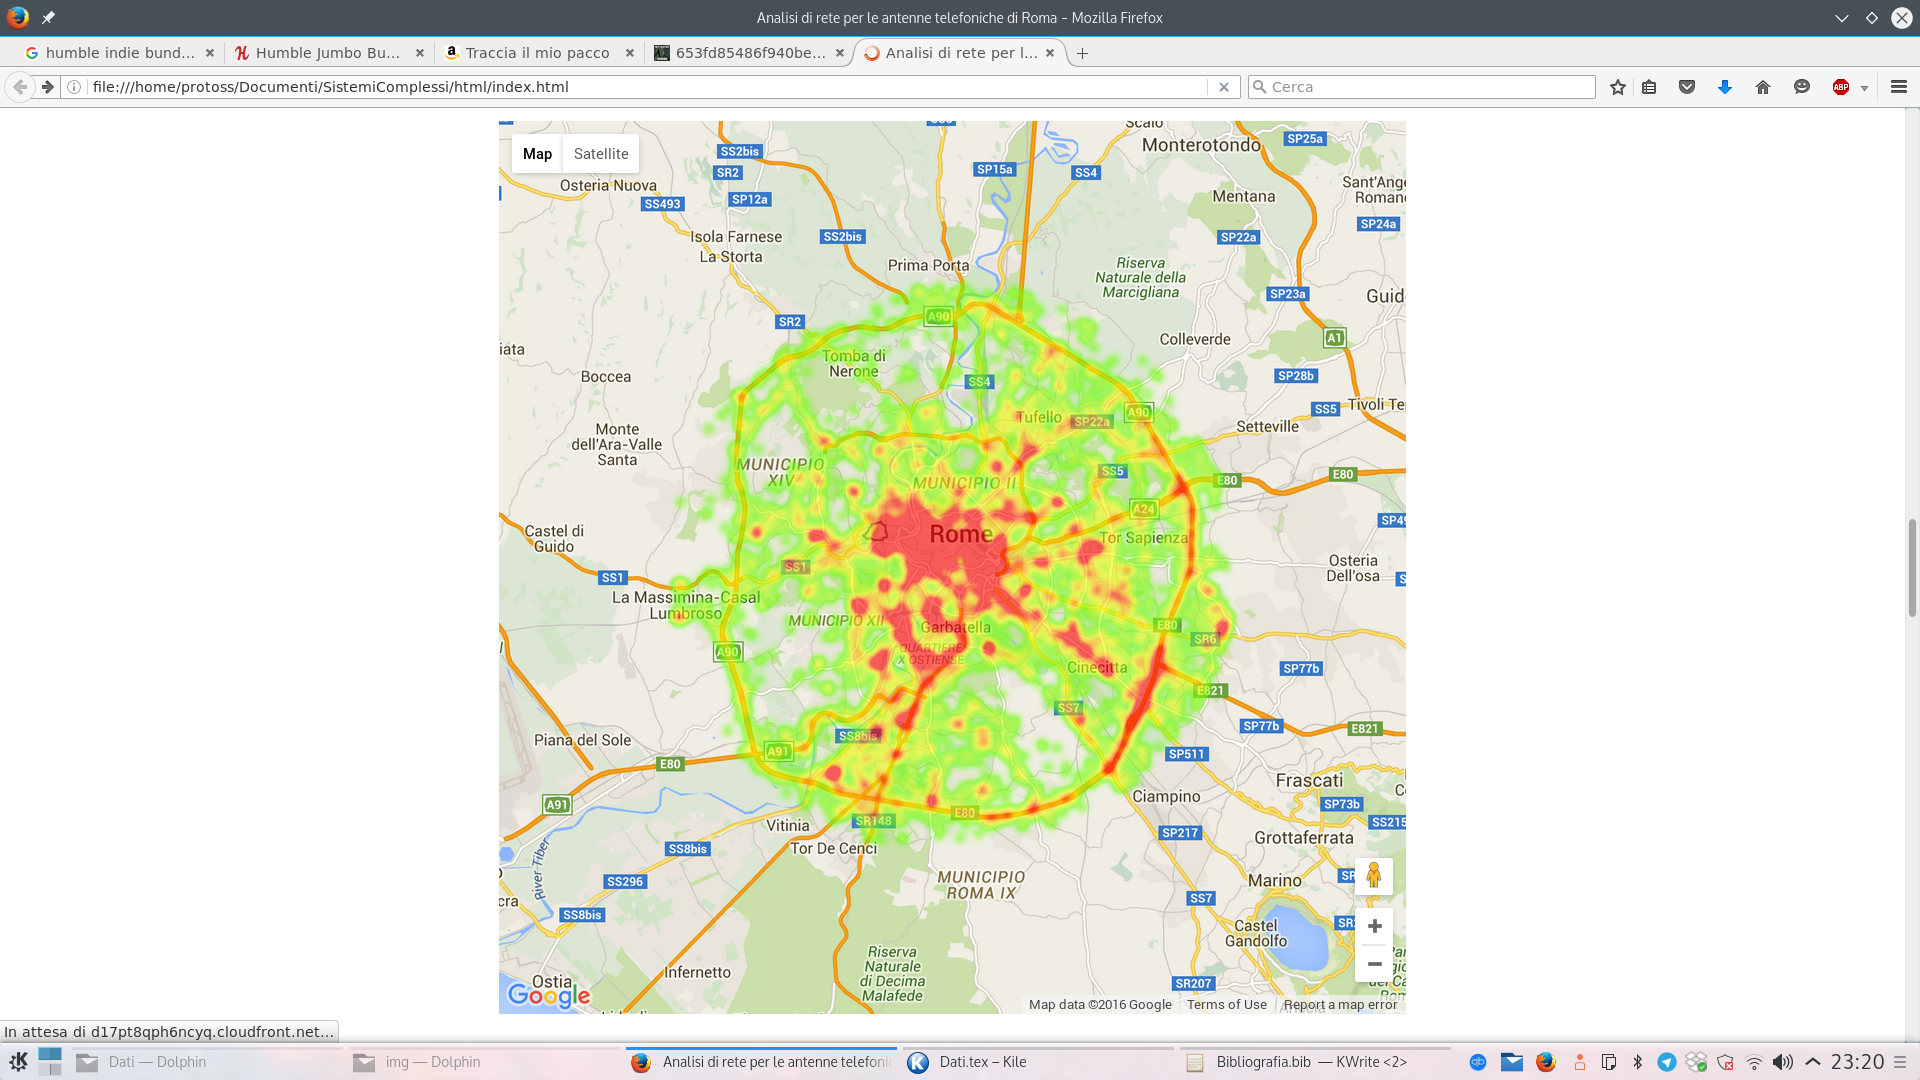
\includegraphics[width=0.46\textwidth]{./Immagini/Dati/Ourmap.png}}
	\caption[Plot antenne.]{Scatterplot e mappa delle antenne telefoniche di roma}
	\label{fig:maps}
\end{figure}

% \clearpage
\subsection{Analisi del raggio di copertura delle antenne}
Dato che ci servirà fare grafici con scale logaritmiche, eliminiamo i dati di antenne che presentano un raggio nullo: \lstinline{range =! 0}

Il raggio minimo risulta essere $1\:m$, mentre quello massimo $41832\:m$. Dato che il raggio del Grande Raccordo Anulare è circa $10\:km$, significa che ci saranno antenne con un grado di connessione totale. Raggi irragionevolmente piccoli probabilmente sono il residuo di misure effettuate con il GPS spento e senza connessione internet, dimodoché il software di acquisizione risulti ingannato assegnando la posizione dell'utente all'antenna più vicina.
% TODO forse spostare questa considerazione a quando si è spiegato il criterio di linking. TODO spiegare la possibile casa di questi valori di raggi così bassi
Facciamo un istogramma log-log per la distribusione del raggio di copertura, sia con la canalizzazione lineare sugli interi, sia con una canalizzazione logaritmica in base 2, per ridurre il rumore sulla coda. La canalizzazione logaritmica pesata permette di osservare l'andamento ben sotto il singolo conteggio, ampliando di una decade l'intervallo di osservazione.

In figura \ref{fig:ranges} si può vedere come l'andamento sia abbastanza power-law su diverse decadi, soprattutto fino a \lstinline{conteggio = 1}. Per verificare ulteriormente questo fatto abbiamo generato anche la curva del \emph{frequency-rank}, che risulta seguire senza esitazioni il trend delineato dagli istogrammi.
%TODO cercare di spiegare questa plaw
Il frequency-rank si ottiene ordinando in maniera decrescente il numero di conteggi per ogni canale unitario e associando un relativo ranking intero decrescente ai raggi corrispondenti. 
 
\begin{figure}[b!]
	\centering
	\subfloat
	{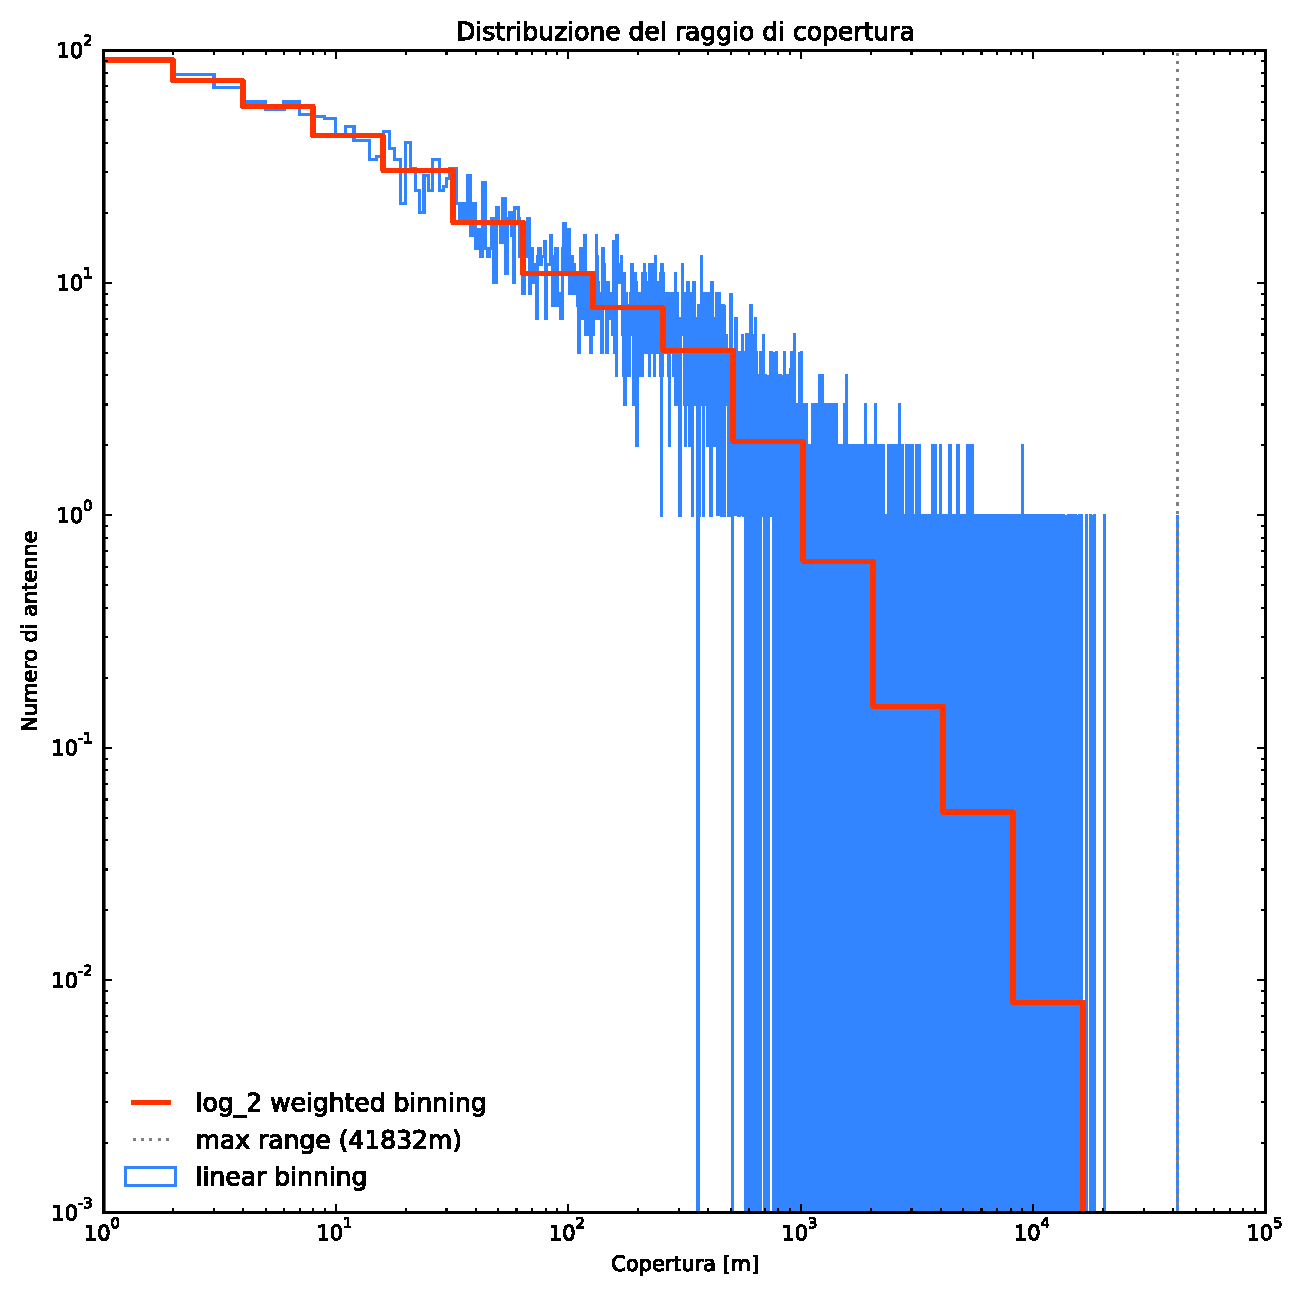
\includegraphics[width=0.48\textwidth]{./Immagini/Dati/logbin}}
	\\
	\subfloat
	{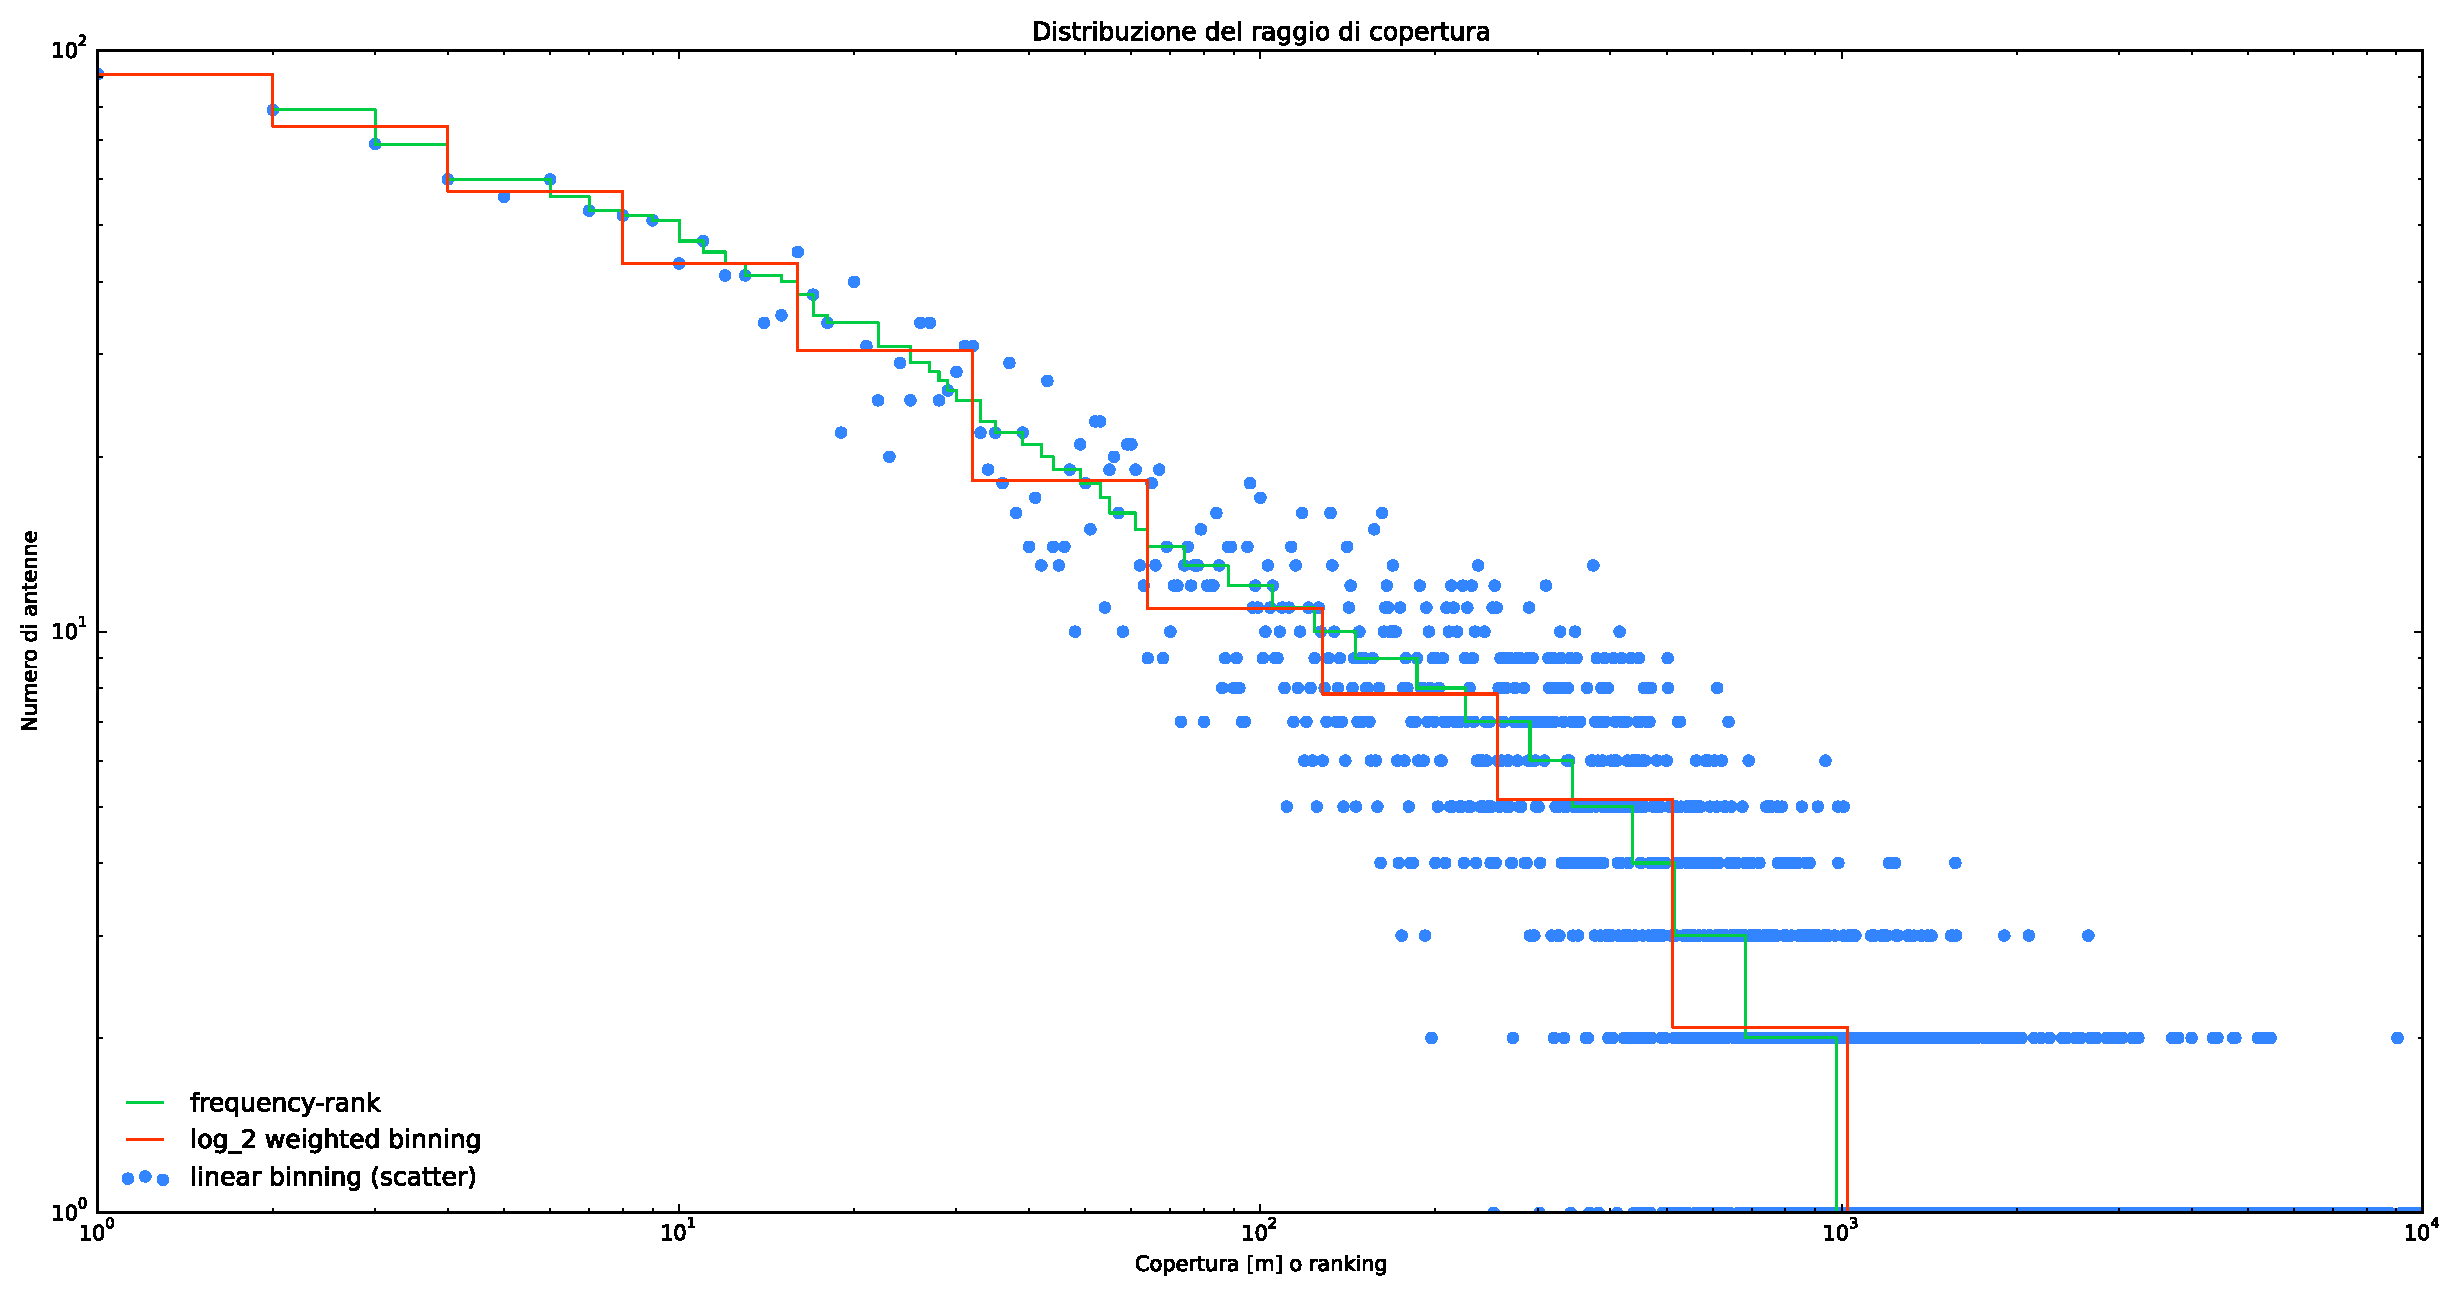
\includegraphics[width=0.6\textwidth]{./Immagini/Dati/rangefreqrank}}
	\caption[Distribuzione raggi.]{Distribuzione e frequency rank dei raggi d'azione delle antenne in scala log-log}
	\label{fig:ranges}
\end{figure} 
 
% Si è infine analizzata la distribuzione cumulata, lasciata nel grafico seguente non normalizzata. La distribuzione cumulata $C(x)$ rappresenta la probabilità che la variabile random assuma un valore minore o uguale a $x$.

% \begin{figure}[ht!]
% 	\centering
% 	\includegraphics[width=0.5\textwidth]{./Immagini/Dati/cumulata}
% 	\caption{Frequency rank dei raggi in scala log-log}
% 	\label{fig:rfreqrank}
% \end{figure}